%\chapter{Conception du projet}
%\label{sec:EnvironnementDeTravail}
\chapter{Analyse fonctionnelle et conceptuelle}
\label{sec:Analyse fonctionnelle et conceptuelle}
%Durant la réalisation de ce projet, nous avons essayé d’utiliser différents
%outils de développement, d’une part afin de rendre la tâche de la
%réalisation plus facile, d’autre part pour que notre système soit robuste et
%répond parfaitement a nos besoins , et que nos interfaces soient claires et
%faciles à utiliser.

%\section{Choix de langage de modélisation :}
\section{Analyse fonctionnelle}
%Dans cette section, je présente le langage et le logiciel de modélisation que j’ai utilisé pour concevoir notre solution.
\begin{comment}
	content...

\subsection{UML}
On a utilisé UML comme langage de modélisation.
Langage de modélisation unifié UML (Unified modeling Langage) un
consiste a modéliser une application logicielle d'une façon standard
dans le cadre de conception orientée objet.
UML consiste a couvrir le cycle de vie d'un logiciel depuis la
spécification des besoins jusqu'au codage en offrant plusieurs
moyens de description et de modélisation des acteurs.
\section{Choix de logiciel de modélisation :}
\subsection{Visual Paradigm  en ligne} 
Visual Paradigm  en ligne est un outil de création de diagrammes en ligne. Vous pouvez créer un nombre illimité de diagrammes, graphiques et autres visuels à partir d’un large éventail de types de diagrammes, y compris UML, organigrammes, BPMN, ERD, DFD, ArchiMate et autres.
%%%%%%%%%%%%%%%%%%%%%%%%%%%%%%%%%%%%%%%%%%%%%%%%%%%%%%%%% Tests %%%%%%%%%%%%%%%%%%%%%%%%%%
\section{Diagramme UML}
\begin{comment}
\begin{table}
		
	\caption{Rôles des diagrammes UML utilisés.}
	\label{table:kysymys}
\begin{tabular}{|c|p{11cm}|}
	
	\hline
	\large \bfseries Diagramme & \large \bfseries Rôle\\
	\hline
	Diagramme de cas d’utilisation & Il consiste à donner une vision globale sur les principales fonctionnalités
	(chaque fonctionnalité représente un cas d’utilisateur) d’une application .  \\
	\hline
	Diagramme d’activité &  Fournir une vue du comportement d'un système en décrivant la séquence d'actions d'un processus.    \\
	\hline
	Diagramme de séquence &Permettent d'identifier les classes requises par un système et le comportement des objets de classes au cours des interactions.  \\
	\hline
	Diagramme de classe    &Le diagramme de classes représente généralement un schéma utilisé en génie
	logiciel pour modéliser un problème bien précis, sous forme des classes et des
	interfaces ainsi que les différentes relations entre celles-ci. \\
	\hline
	
\end{tabular}

\end{table}
\end{comment}
%Table \ref{table:kysymys} on page \pageref{table:kysymys} refers to the ...

\subsection{Diagramme de cas d’utilisation}
\begin{figure}[h!]
	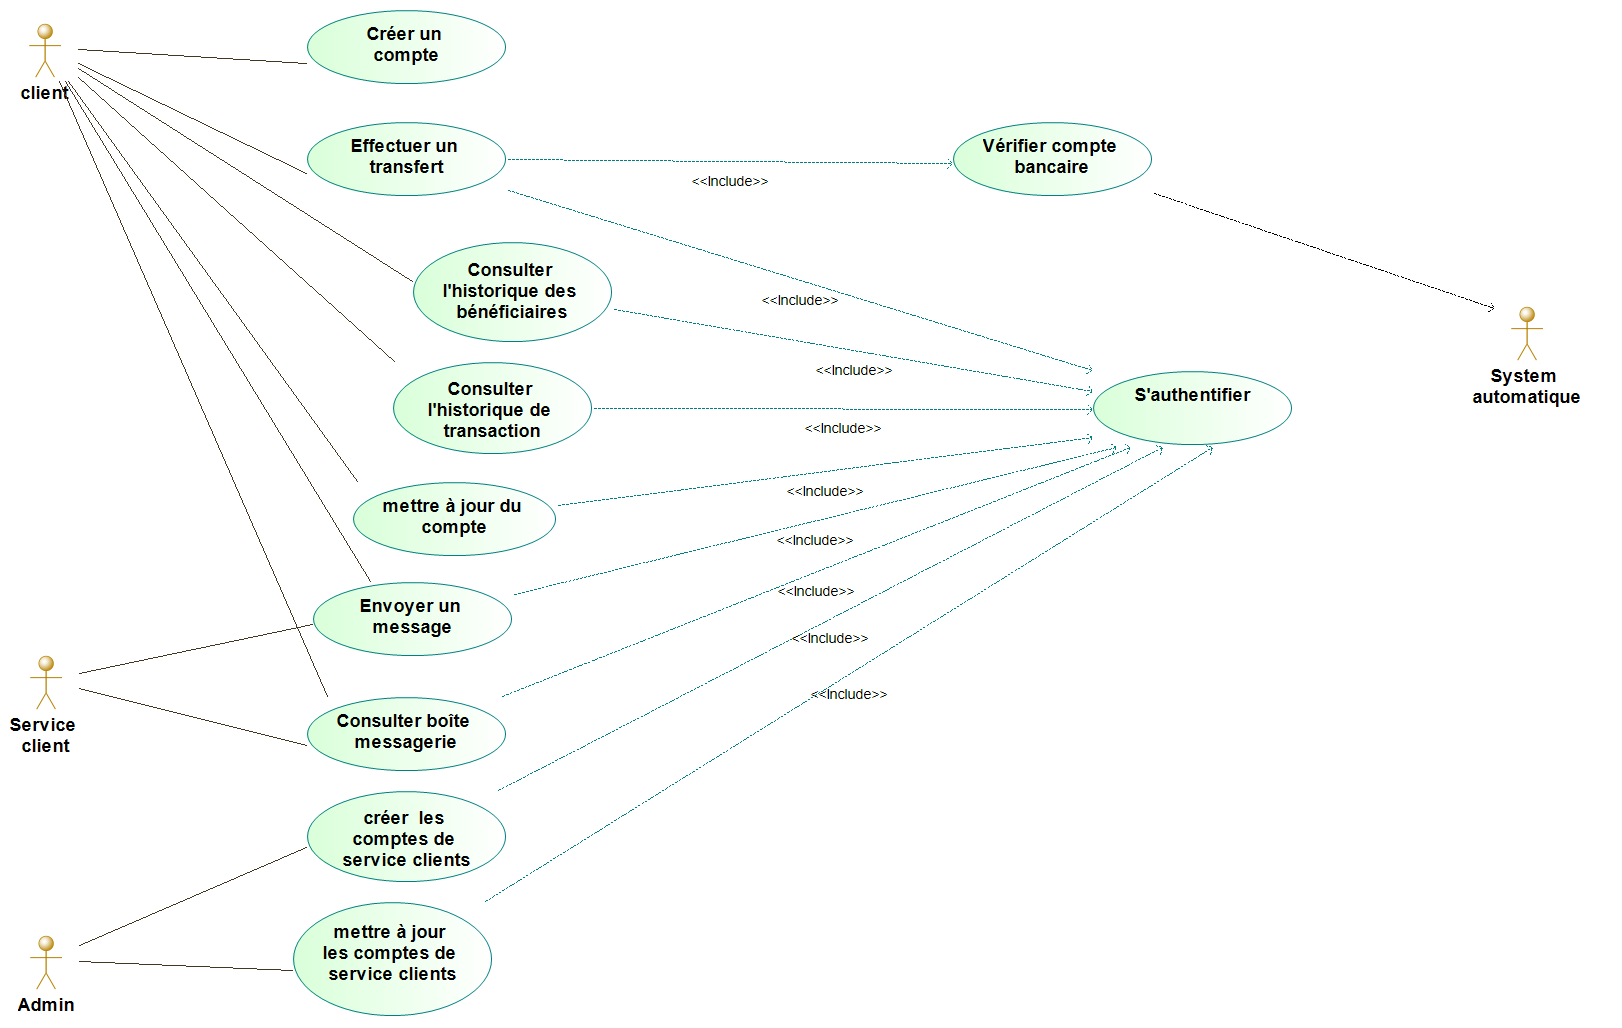
\includegraphics[width=18cm, height=12cm]{./Template LaTeX/Images/use_case.png}
	\caption{Diagramme de cas d’utilisation.}
	\label{fig1:use_case}
\end{figure}
%\textbf{Description détaillée des cas d'utilisation :}
\begin{comment}

\begin{table}[h]
	\begin{tabular}{|m{5cm}|m{2cm}|m{10cm}|}
		\hline
		\textbf{Cas d’utilisation} & \textbf{Acteur} & \textbf{Description}\\
		\hline
		\textbf{Créer un compte }&Client&L'utilisateur se renseigne pour créer un compte au sein de Cadorim pour
		pouvoir accéder au fonctionnalités proposées .\\
		\hline
		\textbf{S’authentifier}&Client&L'utilisateur saisit son identifiant et son mot de passe pour
		accéder aux fonctionnalités.\\
		\hline
		\textbf{Effectuer un transfert}&Client&L'utilisateur saisi le numéro du bénéficiaire et le montant a transférer.
		Une page de vérification avec les informations saisies.
		Transfère le montant vers le bénéficiaire.\\
		\hline
		\textbf{Créer un compte}&Client&L'utilisateur se renseigne pour créer un compte au sein de mauripay pour
		pouvoir accéder au fonctionnalités proposées .\\
		\hline
		\textbf{Créer un compte}&Client&L'utilisateur se renseigne pour créer un compte au sein de mauripay pour
		pouvoir accéder au fonctionnalités proposées .\\
		\hline
		\textbf{Créer un compte}&Client&L'utilisateur se renseigne pour créer un compte au sein de mauripay pour
		pouvoir accéder au fonctionnalités proposées .\\
		\hline
		
	
			
	\end{tabular}
	\caption{Description détaillée des cas d'utilisation}
	\label{4.1}
\end{table}
\end{comment}


	%\textbf{• Description détaillée des cas d'utilisation  :}
\begin{comment}
	
\begin{table}[h]
	\begin{tabular}{|m{4cm}|m{13.5cm}|}
		\hline
		\textbf{Cas d’utilisation}   \textbf{Description}\\
		\hline
		Créer un compte&L'utilisateur se renseigne pour créer un compte au sein de Cadorim pour
		pouvoir accéder au fonctionnalités proposées .\\
		\hline
		S’authentifier&L'utilisateur saisit son identifiant et son mot de passe pour
		accéder aux fonctionnalités.\\
		\hline
		Effectuer un transfert&L'utilisateur saisi le montant a transférer et les informations de  bénéficiaire.
		\newline Une page de vérification avec les informations saisies.
		\newline Transfère le montant vers le bénéficiaire.\\
		\hline
		Consulter l'historique des bénéficaires&L'utilisateur peut voire liste des bénéficaires \\
		\hline
		Consulter l'historique des transactions&L'utilisateur peut voire liste des transactions\\
		\hline
		mettre à jour du compte&L'utilisateur se renseigne pour créer un compte au sein de mauripay pour
		pouvoir accéder au fonctionnalités proposées .\\
		\hline
		Envoyer un message&L'utilisateur se renseigne pour créer un compte au sein de mauripay pour
		pouvoir accéder au fonctionnalités proposées .\\
		\hline
			Consulter boite \newline messagerie&L'utilisateur se renseigne pour créer un compte au sein de mauripay pour
		pouvoir accéder au fonctionnalités proposées .\\
		\hline
		
		
		
	\end{tabular}
	\caption{Description détaillée des cas d'utilisation d'acteur client}
	\label{4.1}
\end{table}
	content...
\end{comment}
%\newpage
\textbf{\hspace*{-1cm}• Description détaillée des cas d'utilisation  :\newline}
\begin{table}[h]
	\hspace*{-2cm}
	\begin{tabular}{|m{19.8cm}|}
		\hline
		\begin{center}
		 \textbf{Cas d’utilisation : Créer un compte, S’authentifier et Créer les comptes de service clients }
		\end{center}
		\\
		[-4ex] 
		\hline
			\begin{tabular}{m{3cm}|m{14cm}}
			
				\centering 	\textbf{Titre} & Créer un compte , S’authentifier , Créer les comptes de service clients
				\\
				[0ex] 
			\end{tabular}
		\\
		
		\hline
			\begin{tabular}{m{3cm}|m{14cm}}
			
			\centering 	\textbf{But} & Créer un compte pour accéder aux fonctionnalités de l’application 	\\
			[0ex] 
			
		\end{tabular}
		\\
		\hline
			\begin{tabular}{m{3cm}|m{15.5cm}}
			
			\centering 	\textbf{Résumé} & L'utilisateur doit remplir un formulaire d’inscription et identifier électroniquement leur document comme des pièces d’identité (carte d’identité, passeport ) à partir de leur caméra du téléphone puis valide son action.\newline Le système effectue une vérification puis une mise à jour de la base de données.
			\\
			[0ex] 
		\end{tabular}
		\\
		
		\hline
			\begin{tabular}{m{3cm}|m{14cm}}
			
			\centering 	\textbf{Acteurs } & Client,Admin \\[0ex]
			
		\end{tabular}
		\\
		 
		\hline
		\begin{center}
			\textbf{Descriptions des enchainements}
		\end{center}
		\\
		[-4ex] 
		\hline	
			\begin{tabular}{m{9.3cm}|m{9.3cm}}
			
			\begin{center}
				\textbf{Pré condition}
			\end{center}
		 		& 
		 	\begin{center}
				\textbf{Post condition}
			\end{center}
			\\[-4ex]
		\end{tabular}
		\\
		
		\hline
			\begin{tabular}{m{9.3cm}|m{9.3cm}}
			L'utilisateur doit accéder au système
			& 
			L'utilisateur inscrit
		\end{tabular}
		\\
		\hline
			\begin{center}
			\textbf{Scenario nominal}
			\end{center}
		\\
		[-4ex]
		\hline
		\begin{enumerate}
			\item [1.] L’utilisateur demande la page d’inscription en cliquant sur «S'INSCRIRE»
			\item [2.] Le système lui envoie la page d’inscription
			\item [3.] L’utilisateur rempli le formulaire et scanne leur document puis appuie sur S'INSCRIRE
			\item [4.] Le système effectue les validations et l’enregistrement dans la base de données
			\item [5.] L’utilisateur est redirigé vers la page d’authentification et renseigne ses identifiants en cas d'acteur client 
		\end{enumerate}
		\\
		[-4ex]
		\hline	
			\begin{center}
			\textbf{Enchainement d’échec }
		\end{center}
		\\ 
		[-4ex]
		\hline
		\begin{tabular}{m{17.5cm}}
			\begin{enumerate}
				\item [6.] Le compte existe déjà ou les données saisies sont incorrectes
				\item [7.] Il n’y a pas de connexion internet
			\end{enumerate}
			\\[-4ex]
		\end{tabular}
		\\
		\hline	
		
	\end{tabular}
	\centering \caption{Description détaillée des cas d'utilisation : Créer un compte  et S’authentifier}
	\label{4.1}
\end{table}
\newpage

\begin{table}[h]
	\hspace*{-2cm}
	\vspace*{-2cm}
	\begin{tabular}{|m{19.8cm}|}
		\hline
		\begin{center}
			\textbf{Cas d’utilisation : Effectuer transfert}
		\end{center}
		\\
		[-4ex] 
		\hline
		\begin{tabular}{m{3cm}|m{14cm}}
			
			\centering 	\textbf{Titre} & Effectuer transfert
			\\
			[0ex] 
		\end{tabular}
		\\
		
		\hline
		\begin{tabular}{m{3cm}|m{14cm}}
			
			\centering 	\textbf{But} & Envoyer de l’argent à un bénéficiaire	\\
			[0ex] 
			
		\end{tabular}
		\\
		\hline
		\begin{tabular}{m{3cm}|m{15.5cm}}
			
			\centering 	\textbf{Résumé} & L’utilisateur saisit les informations du bénéficiaire et le montant de la transaction et valide. Le système envoyait les informations de la carte bancaire au  fournisseur de paiement  avant de finaliser l’opération.
			\\
			[0ex] 
		\end{tabular}
		\\
		
		\hline
		\begin{tabular}{m{3cm}|m{14cm}}
			
			\centering 	\textbf{Acteurs } & Client \\[0ex]
			
		\end{tabular}
		\\
		
		\hline
		\begin{center}
			\textbf{Descriptions des enchainements}
		\end{center}
		\\
		[-4ex] 
		\hline	
		\begin{tabular}{m{9.3cm}|m{9.3cm}}
			
			\begin{center}
				\textbf{Pré condition}
			\end{center}
			& 
			\begin{center}
				\textbf{Post condition}
			\end{center}
			\\[-4ex]
		\end{tabular}
		\\
		
		\hline
		\begin{tabular}{m{9.3cm}|m{9.3cm}}
			- L’utilisateur doit se connecter \newline
			- L’utilisateur doit utiliser une carte bancaire valide & 
			- Le transfert est effectué \newline
			- Afficher  l'historique des transactions
			\\[0ex]
		\end{tabular}
		\\
		\hline
		\begin{center}
			\textbf{Scenario nominal}
		\end{center}
		\\
		[-4ex]
		\hline
		\begin{enumerate}
			\item [1.] L’utilisateur accède au formulaire de transfert en saisit le montant puis  cliquant sur « Envoyer »
			\item [2.] Le système lui demande de saisir les informations de transfert
			\item [3.] L’utilisateur rempli le formulaire appuie sur le bouton « Valider »
			\item [4.] Le système débiter le compte de cadorim et crédité le compte de bénéficiaire
			\item [5.] Le système lui affiche la page de l'historique des transactions
		\end{enumerate}
		\\
		[-4ex]
		\hline	
		\begin{center}
			\textbf{Enchainement d’échec }
		\end{center}
		\\ 
		[-4ex]
		\hline
		\begin{tabular}{m{17.5cm}}
			\begin{enumerate}
				\item [6.] La carte bancaire invalide ou le solde est insuffisant
				\item [7.] La saisie de données n’est pas correcte
				\item [8.] La connexion n’est pas bonne pour effectuer et suivre un transfert
			\end{enumerate}
			\\[-4ex]
		\end{tabular}
		\\
		\hline	
		
	\end{tabular}
	\vspace*{1.5cm}
	\centering \caption{Description détaillée des cas d'utilisation : Effectuer transfert}
	\label{4.1}
\end{table}

\newpage

\begin{table}[h]
	\hspace*{-2cm}
	\vspace*{-2.5cm}
	\begin{tabular}{|m{19.8cm}|}
		\hline
		\begin{center}
			\textbf{Cas d’utilisation : Consulter l'historique des bénéficiaires et l'historique de transaction}
		\end{center}
		\\
		[-4ex] 
		\hline
		\begin{tabular}{m{3cm}|m{14cm}}
			
			\centering 	\textbf{Titre} & Consulter l'historique des bénéficiaires,Consulter l'historique de transaction
			\\
			[0ex] 
		\end{tabular}
		\\
		
		\hline
		\begin{tabular}{m{3cm}|m{14cm}}
			
			\centering 	\textbf{But} & Consultations de l'historique\\
			[0ex] 
			
		\end{tabular}
		\\
		\hline
		\begin{tabular}{m{3cm}|m{15.5cm}}
			
			\centering 	\textbf{Résumé} & L'utilisateur voit les renseignements sur le bénéficiaire et l'opération de transaction.
			\\
			[0ex] 
		\end{tabular}
		\\
		
		\hline
		\begin{tabular}{m{3cm}|m{14cm}}
			
			\centering 	\textbf{Acteurs } & Client \\[0ex]
			
		\end{tabular}
		\\
		
		\hline
		\begin{center}
			\textbf{Descriptions des enchainements}
		\end{center}
		\\
		[-4ex] 
		\hline	
		\begin{tabular}{m{9.3cm}|m{9.3cm}}
			
			\begin{center}
				\textbf{Pré condition}
			\end{center}
			& 
			\begin{center}
				\textbf{Post condition}
			\end{center}
			\\[-4ex]
		\end{tabular}
		\\
		
		\hline
		\begin{tabular}{m{9.3cm}|m{9.3cm}}
			- L’utilisateur doit se connecter \newline
			 & 
			- Afficher  l'historique des transactions ou des  \newline bénéficiaires
			\\[0ex]
		\end{tabular}
		\\
		\hline
		\begin{center}
			\textbf{Scenario nominal}
		\end{center}
		\\
		[-4ex]
		\hline
		\begin{enumerate}
			\item [1.] L’utilisateur accède a l'historique des transactions ou des bénéficiaires en cliquant sur « Transferts » ou « Benef »
			\item [2.] Le système lui affiche la page de l'historique
		\end{enumerate}
		\\
		[-4ex]
		\hline	
		\begin{center}
			\textbf{Enchainement d’échec }
		\end{center}
		\\ 
		[-4ex]
		\hline
		\begin{tabular}{m{17.5cm}}
			\begin{enumerate}
				\item [3.] Il n’y a pas de connexion internet
				
			\end{enumerate}
			\\[-4ex]
		\end{tabular}
		\\
		\hline	
		
	\end{tabular}
	\vspace*{2cm}
	\centering \caption{Description détaillée des cas d'utilisation : Consulter l'historiques(des transactions ou des bénéficiaires)}
	\label{4.1}
\end{table}

\newpage

\begin{table}[h]
	\hspace*{-2cm}
	\vspace*{-2cm}
	\begin{tabular}{|m{19.8cm}|}
		\hline
		\begin{center}
			\textbf{Cas d’utilisation : Consulter boite messagerie}
		\end{center}
		\\
		[-4ex] 
		\hline
		\begin{tabular}{m{3cm}|m{14cm}}
			
			\centering 	\textbf{Titre} & Consulter boite messagerie
			\\
			[0ex] 
		\end{tabular}
		\\
		
		\hline
		\begin{tabular}{m{3cm}|m{14cm}}
			
			\centering 	\textbf{But} & Consulter boite messagerie\\
			[0ex] 
			
		\end{tabular}
		\\
		\hline
		\begin{tabular}{m{3cm}|m{15.5cm}}
			
			\centering 	\textbf{Résumé} &L'utilisateur voit l'historique des  messages et les messages reçus.
			\\
			[0ex] 
		\end{tabular}
		\\
		
		\hline
		\begin{tabular}{m{3cm}|m{14cm}}
			
			\centering 	\textbf{Acteurs } & Client, Srvice client \\[0ex]
			
		\end{tabular}
		\\
		
		\hline
		\begin{center}
			\textbf{Descriptions des enchainements}
		\end{center}
		\\
		[-4ex] 
		\hline	
		\begin{tabular}{m{9.3cm}|m{9.3cm}}
			
			\begin{center}
				\textbf{Pré condition}
			\end{center}
			& 
			\begin{center}
				\textbf{Post condition}
			\end{center}
			\\[-4ex]
		\end{tabular}
		\\
		
		\hline
		\begin{tabular}{m{9.3cm}|m{9.3cm}}
			- L’utilisateur doit se connecter \newline
			& 
			- Afficher  l'historique des  messages et les messages reçus
			\\[0ex]
		\end{tabular}
		\\
		\hline
		\begin{center}
			\textbf{Scenario nominal}
		\end{center}
		\\
		[-4ex]
		\hline
		\begin{enumerate}
			\item [1.] L’utilisateur accède à la boîte messagerie
			\item [2.] Le système lui affiche la page des messageries
		\end{enumerate}
		\\
		[-4ex]
		\hline	
		\begin{center}
			\textbf{Enchainement d’échec }
		\end{center}
		\\ 
		[-4ex]
		\hline
		\begin{tabular}{m{17.5cm}}
			\begin{enumerate}
				\item [3.] Il n’y a pas de connexion internet
				
			\end{enumerate}
			\\[-4ex]
		\end{tabular}
		\\
		\hline	
		
	\end{tabular}
	\vspace*{1.5cm}
	\centering \caption{Description détaillée des cas d'utilisation : Consulter boite messagerie}
	\label{4.1}
\end{table}


\newpage

\begin{table}[h]
	\hspace*{-2cm}
	\vspace*{-2cm}
	\begin{tabular}{|m{19.8cm}|}
		\hline
		\begin{center}
			\textbf{Cas d’utilisation : Envoyer un message}
		\end{center}
		\\
		[-4ex] 
		\hline
		\begin{tabular}{m{3cm}|m{14cm}}
			
			\centering 	\textbf{Titre} & Envoyer un message
			\\
			[0ex] 
		\end{tabular}
		\\
		
		\hline
		\begin{tabular}{m{3cm}|m{14cm}}
			
			\centering 	\textbf{But} & Envoyer un message\\
			[0ex] 
			
		\end{tabular}
		\\
		\hline
		\begin{tabular}{m{3cm}|m{15.5cm}}
			
			\centering 	\textbf{Résumé} &L'utilisateur peut envoyer un message où répond à un message
			\\
			[0ex] 
		\end{tabular}
		\\
		
		\hline
		\begin{tabular}{m{3cm}|m{14cm}}
			
			\centering 	\textbf{Acteurs } & Client, Srvice client \\[0ex]
			
		\end{tabular}
		\\
		
		\hline
		\begin{center}
			\textbf{Descriptions des enchainements}
		\end{center}
		\\
		[-4ex] 
		\hline	
		\begin{tabular}{m{9.3cm}|m{9.3cm}}
			
			\begin{center}
				\textbf{Pré condition}
			\end{center}
			& 
			\begin{center}
				\textbf{Post condition}
			\end{center}
			\\[-4ex]
		\end{tabular}
		\\
		
		\hline
		\begin{tabular}{m{9.3cm}|m{9.3cm}}
			- L’utilisateur doit se connecter \newline
			& 
			\centering - Le message est envoyé
			\\[0ex]
		\end{tabular}
		\\
		\hline
		\begin{center}
			\textbf{Scenario nominal}
		\end{center}
		\\
		[-4ex]
		\hline
		\begin{enumerate}
			\item [1.] L’utilisateur demande le formulaire d’envoi de message
			\item [2.] Le système lui affiche la page des discussions
		\end{enumerate}
		\\
		[-4ex]
		\hline	
		\begin{center}
			\textbf{Enchainement d’échec }
		\end{center}
		\\ 
		[-4ex]
		\hline
		\begin{tabular}{m{17.5cm}}
			\begin{enumerate}
				\item [3.] Il n’y a pas de connexion internet
				
			\end{enumerate}
			\\[-4ex]
		\end{tabular}
		\\
		\hline	
		
	\end{tabular}
	\vspace*{1.5cm}
	\centering \caption{Description détaillée des cas d'utilisation : Envoyer un message}
	\label{4.1}
\end{table}
\begin{comment}

	\item[•]  \textbf{Description détaillée des cas d'utilisation d'acteur service client :}
\begin{table}[h]
	\begin{tabular}{|m{4cm}|m{13.5cm}|}
		\hline
		\textbf{Cas d’utilisation}  & \textbf{Description}\\
		\hline
		Enoyer un message&L'utilisateur se renseigne pour créer un compte au sein de Cadorim pour
		pouvoir accéder au fonctionnalités proposées .\\
		\hline
		S’authentifier&L'utilisateur saisit son identifiant et son mot de passe pour
		accéder aux fonctionnalités.\\
		\hline
			Consulter boite \newline messagerie&L'utilisateur saisit son identifiant et son mot de passe pour
		accéder aux fonctionnalités.\\
		\hline
	\end{tabular}
	\caption{Description détaillée des cas d'utilisation d'acteur service client}
	\label{4.1}
\end{table}

	\item[•]  \textbf{Description détaillée des cas d'utilisation d'acteur admin :}
\begin{table}[h]
	\begin{tabular}{|m{4cm}|m{13.5cm}|}
		\hline
		\textbf{Cas d’utilisation}  & \textbf{Description}\\
		\hline
		Créer les comptes de service clients&L'utilisateur se renseigne pour créer un compte au sein de Cadorim pour
		pouvoir accéder au fonctionnalités proposées .\\
		\hline
		S’authentifier&L'utilisateur saisit son identifiant et son mot de passe pour
		accéder aux fonctionnalités.\\
		\hline
		Mettre à jour les comptes de service clients&L'utilisateur saisit son identifiant et son mot de passe pour
		accéder aux fonctionnalités.\\
		\hline
	\end{tabular}
	\caption{Description détaillée des cas d'utilisation d'acteur admin}
	\label{4.1}
\end{table}
\item[•]  \textbf{Description détaillée des cas d'utilisation d'acteur system :}
\begin{table}[h]
	\begin{tabular}{|m{4cm}|m{13.5cm}|}
		\hline
		\textbf{Cas d’utilisation}  & \textbf{Description}\\
		\hline
		 Vérifier compte \newline bancaire&L'utilisateur se renseigne pour créer un compte au sein de Cadorim pour
		pouvoir accéder au fonctionnalités proposées .\\
		\hline
	\end{tabular}
	\caption{Description détaillée des cas d'utilisation d'acteur secondaire system}
	\label{4.1}
\end{table}
	content...
\end{comment}


\subsection{Diagramme d’activité}
Cette section a pour objectif de mettre en surbrillance le processus quelques fonctionnalités de
l’application pour voir les détailles. J’ai choisi trois cas d’utilisation, à savoir, la création d’un compte,la transfert d'argent et l'authentification.
\newpage
\subsubsection{Création de compte}
Le diagramme d’activité qu’illustre la figure~\ref{activiteCompte} décrit le cas d’utilisation « Créer un compte ».
\begin{figure}[h!]
	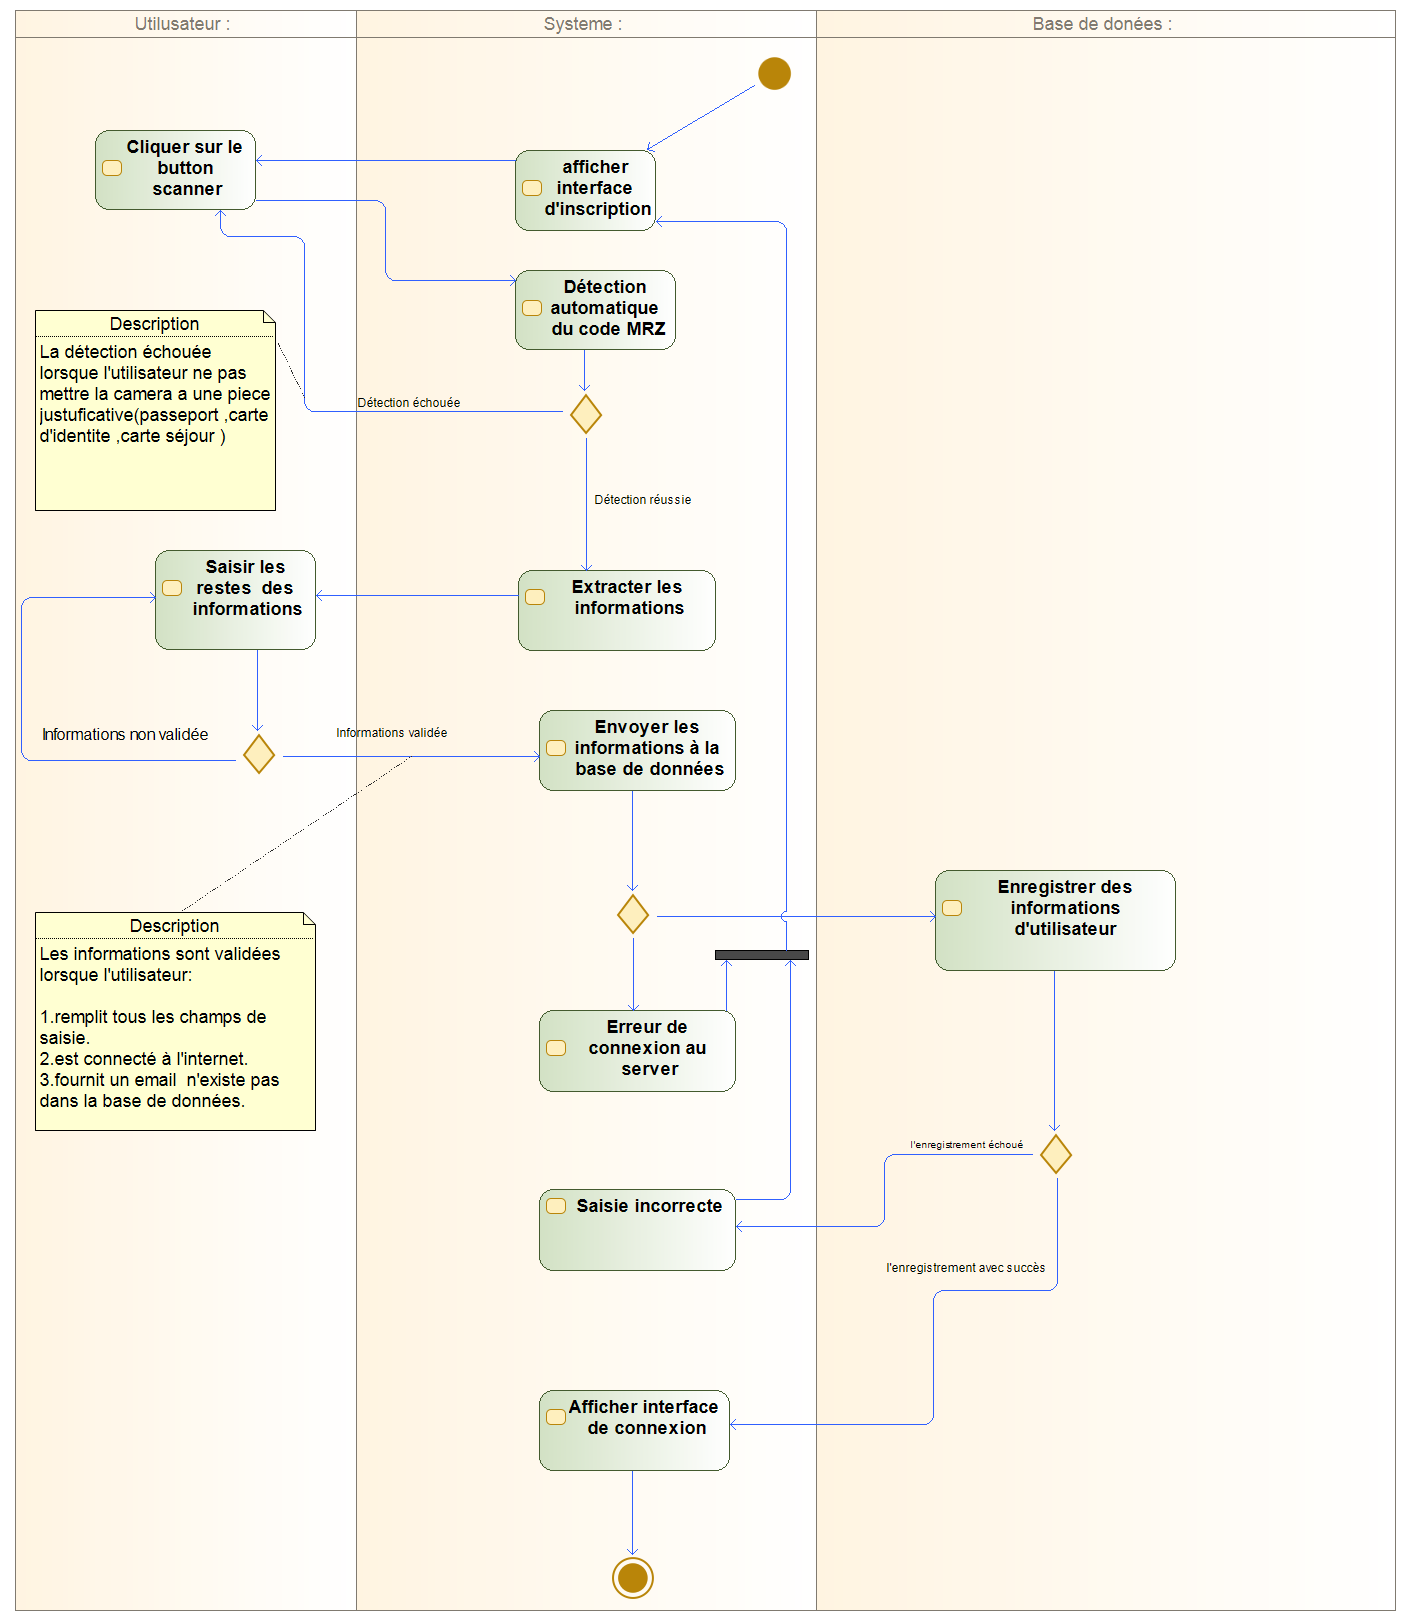
\includegraphics[width=18cm, height=19cm]{./Template LaTeX/Images/ins_act.png}
\caption{Diagramme d’activité : Création de compte}
\label{activiteCompte}

\end{figure}

\subsubsection{Transfert d'argent}
Le diagramme d’activité qu’illustre la figure~\ref{activiteTr} décrit les différentes actions ou enchainements
effectués lors d’une opération de transfert d’argent.
\begin{figure}[h!]
	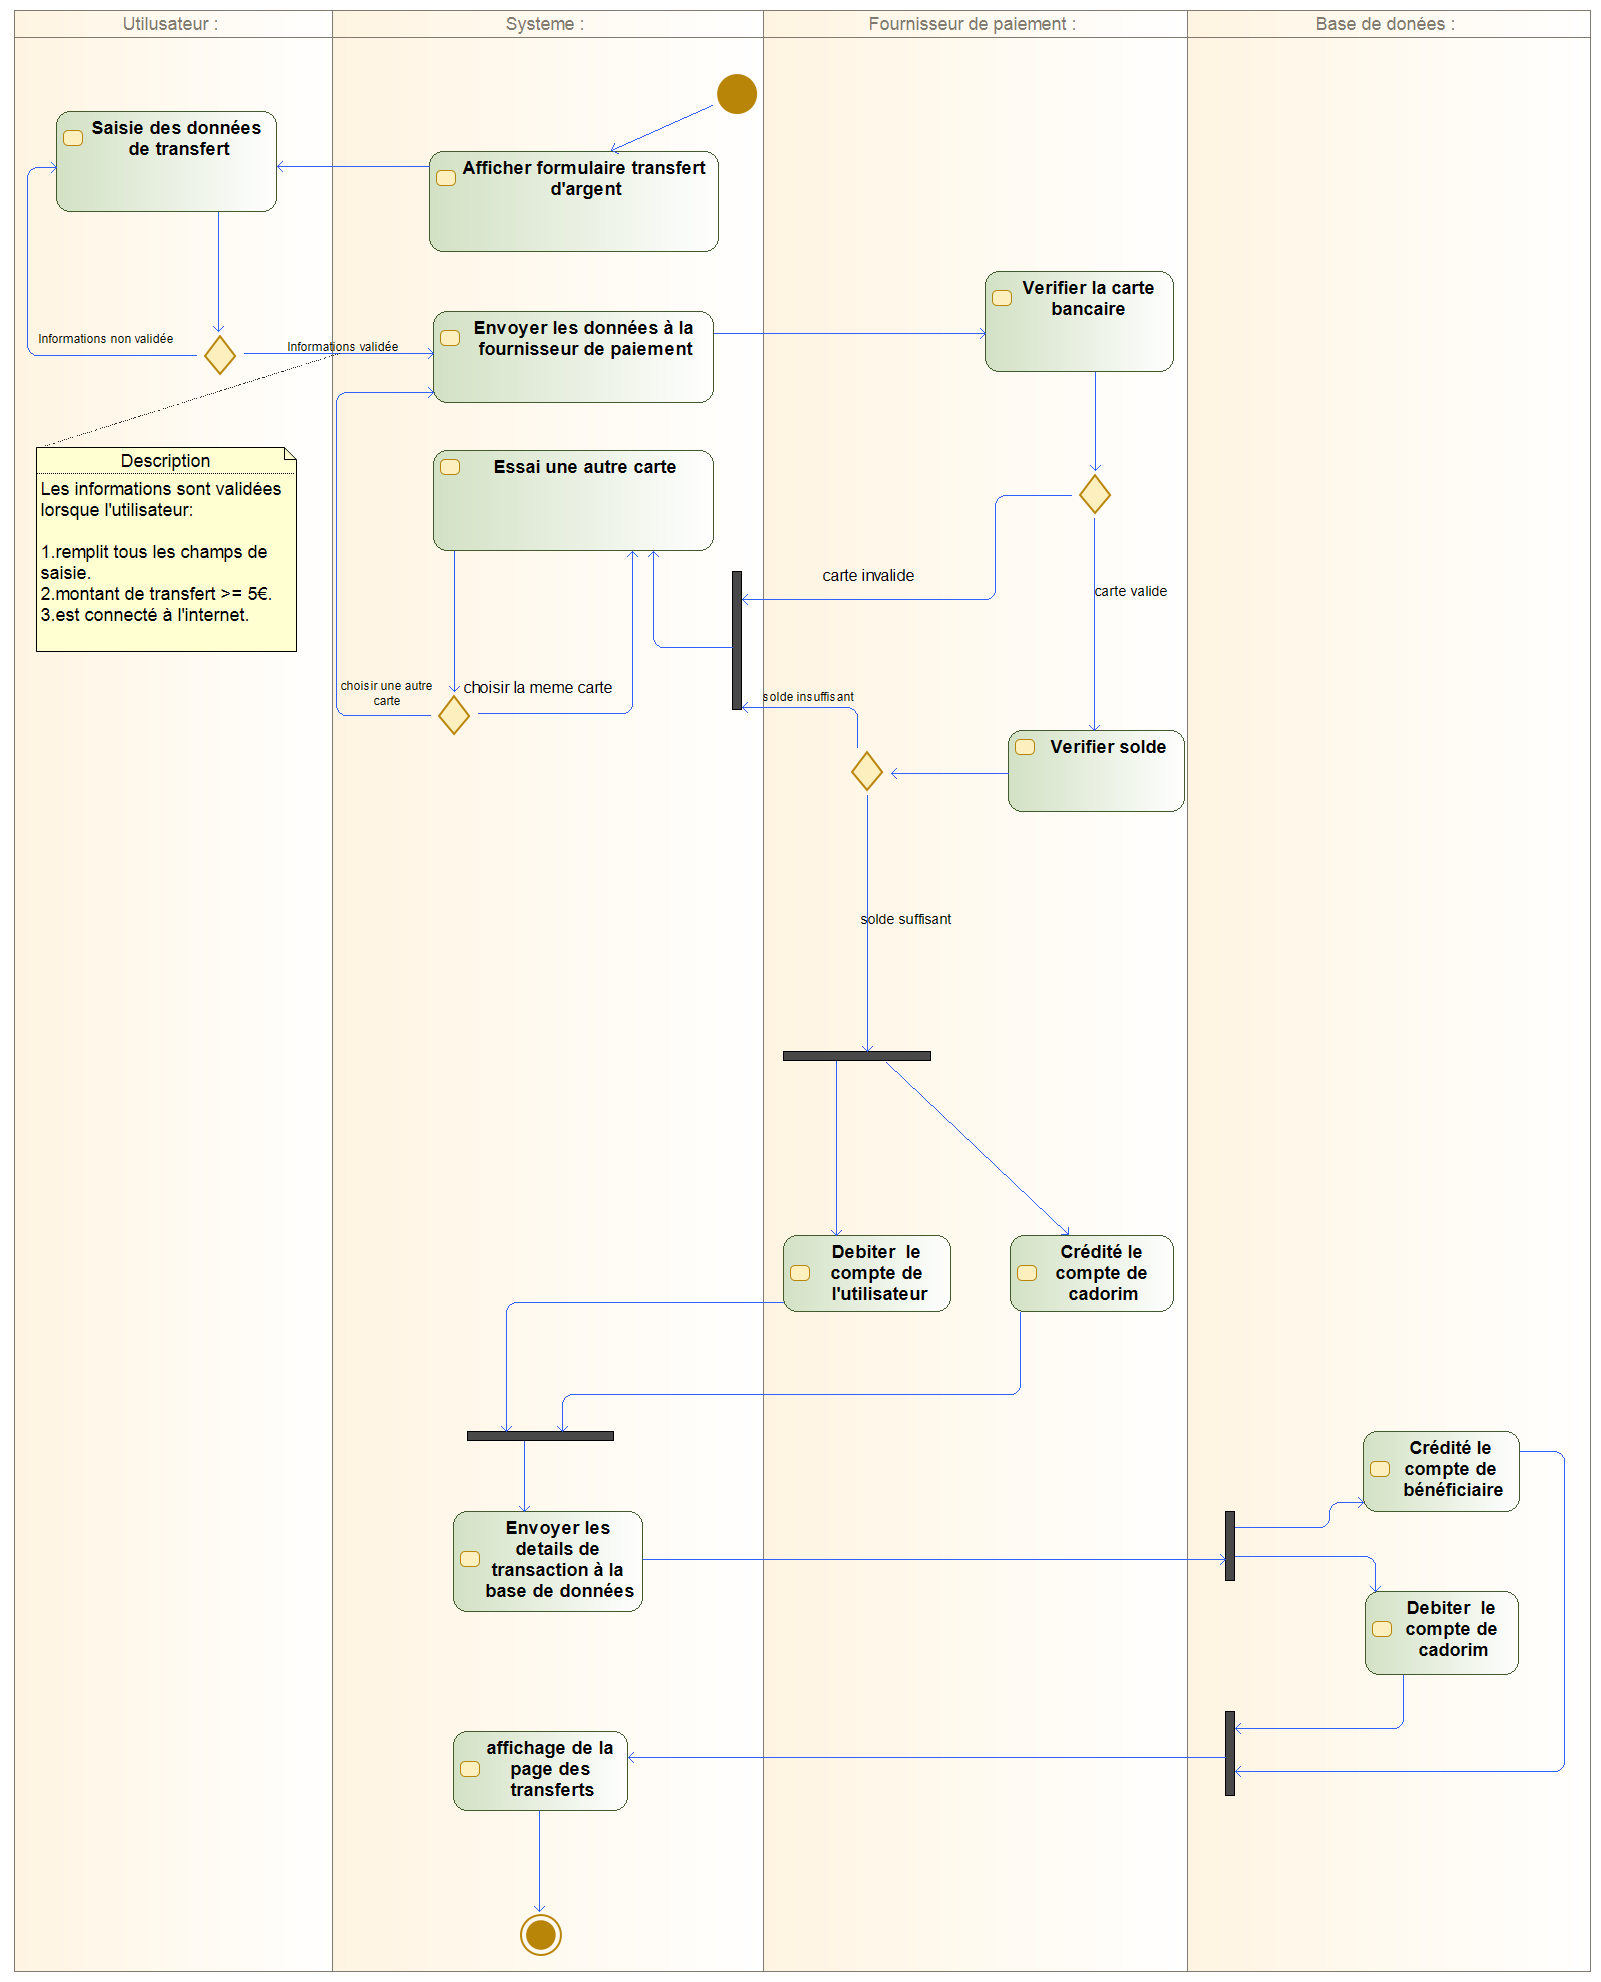
\includegraphics[width=18cm, height=20cm]{./Template LaTeX/Images/trans_act.png}
	\caption{Diagramme d'activité : Transfert d'argent}
	\label{activiteTr}
\end{figure}

\subsubsection{Authentification}
Le diagramme d’activité qu’illustre la figure~\ref{activiteAuth} décrit le cas d’utilisation « Authentification ».
\begin{figure}[h!]
	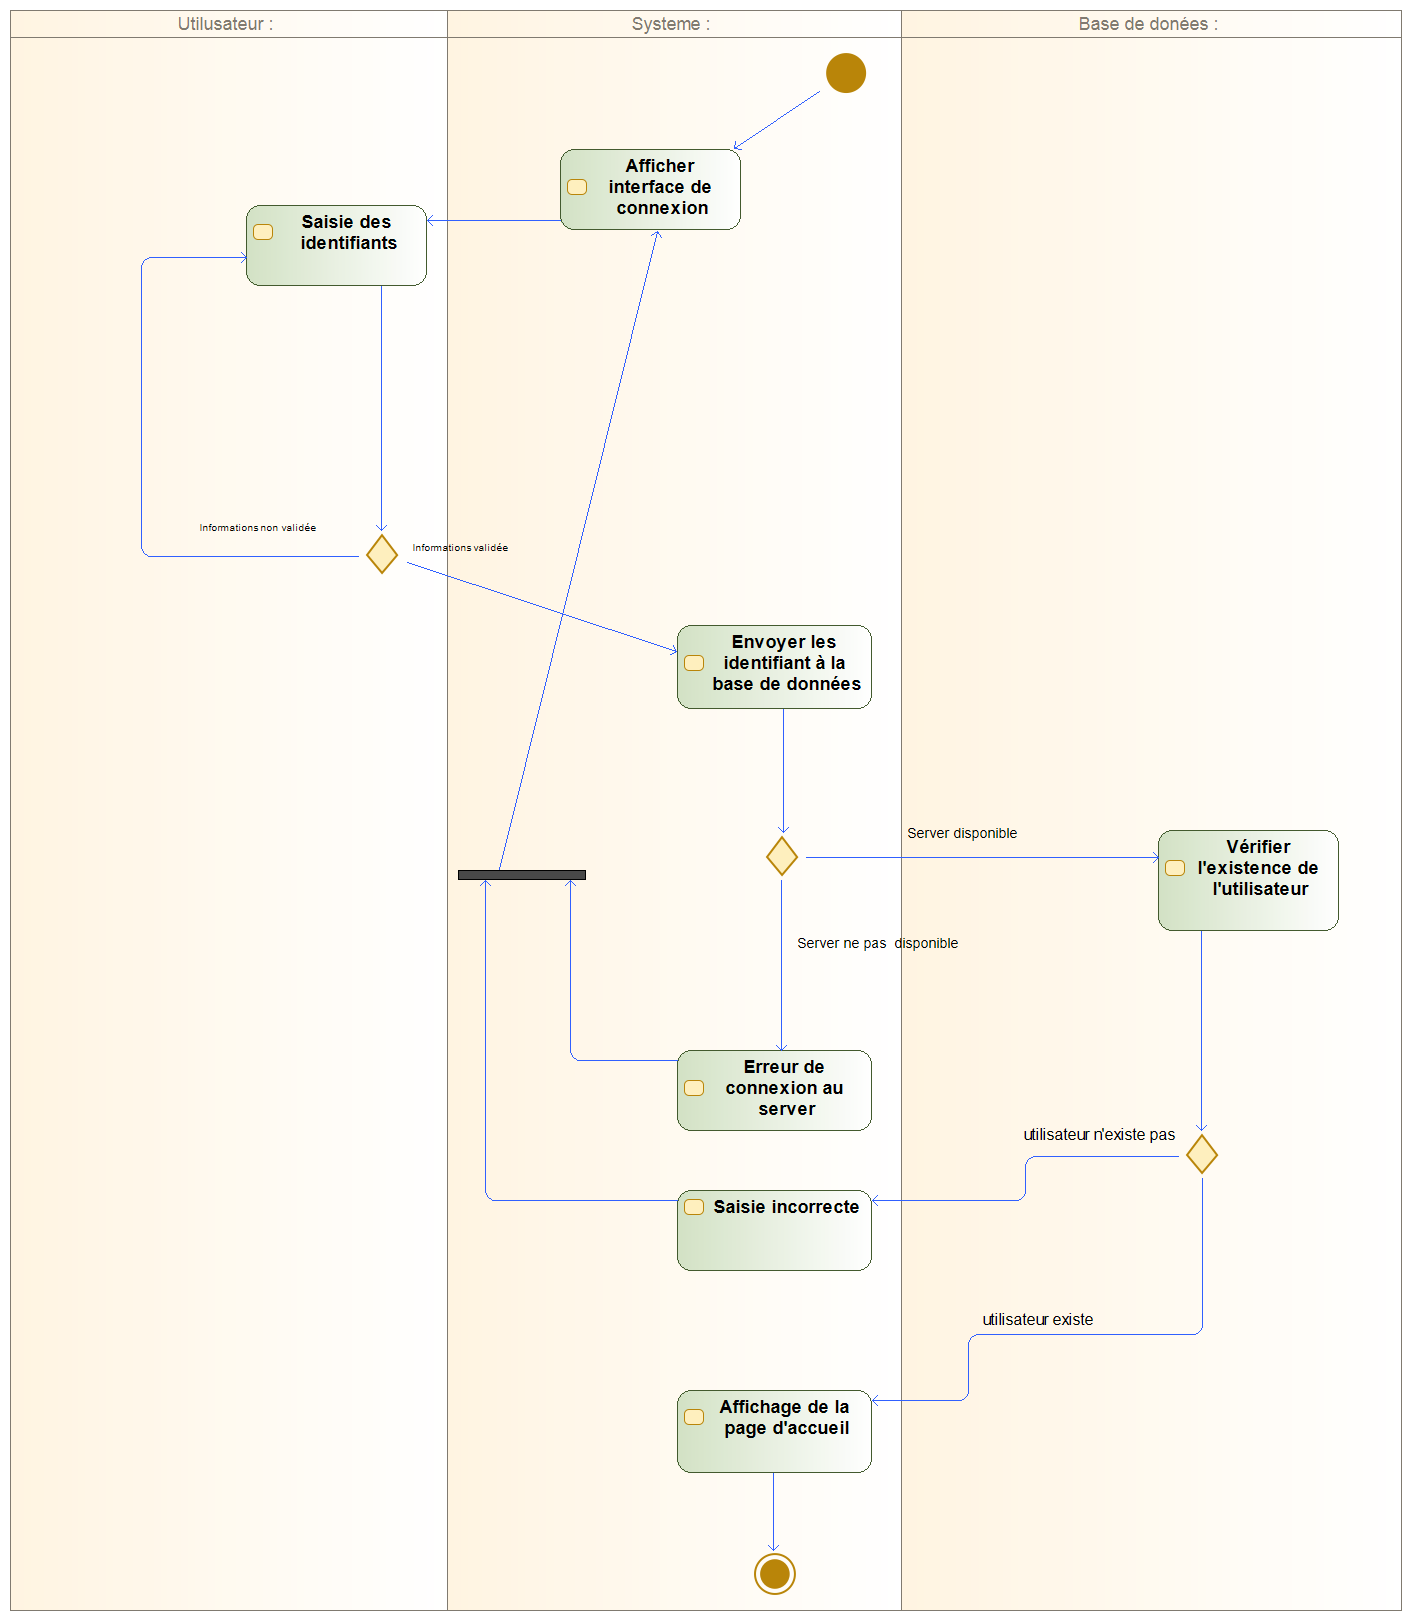
\includegraphics[width=18cm, height=20cm]{./Template LaTeX/Images/auth_act.png}
	\caption{Diagramme d'activité : Authentification}
	\label{activiteAuth}
\end{figure}


%\section{Modélisation de la base de données}
%\subsection{Diagramme de séquence}
%\newpage

\subsection{Diagramme de classe}
Afin de bien détailler l’architecture de la base de données, nous avons conçu le diagramme de
classe représenté dans la figure~\ref{fig4:class}.
\begin{figure}[h!]
	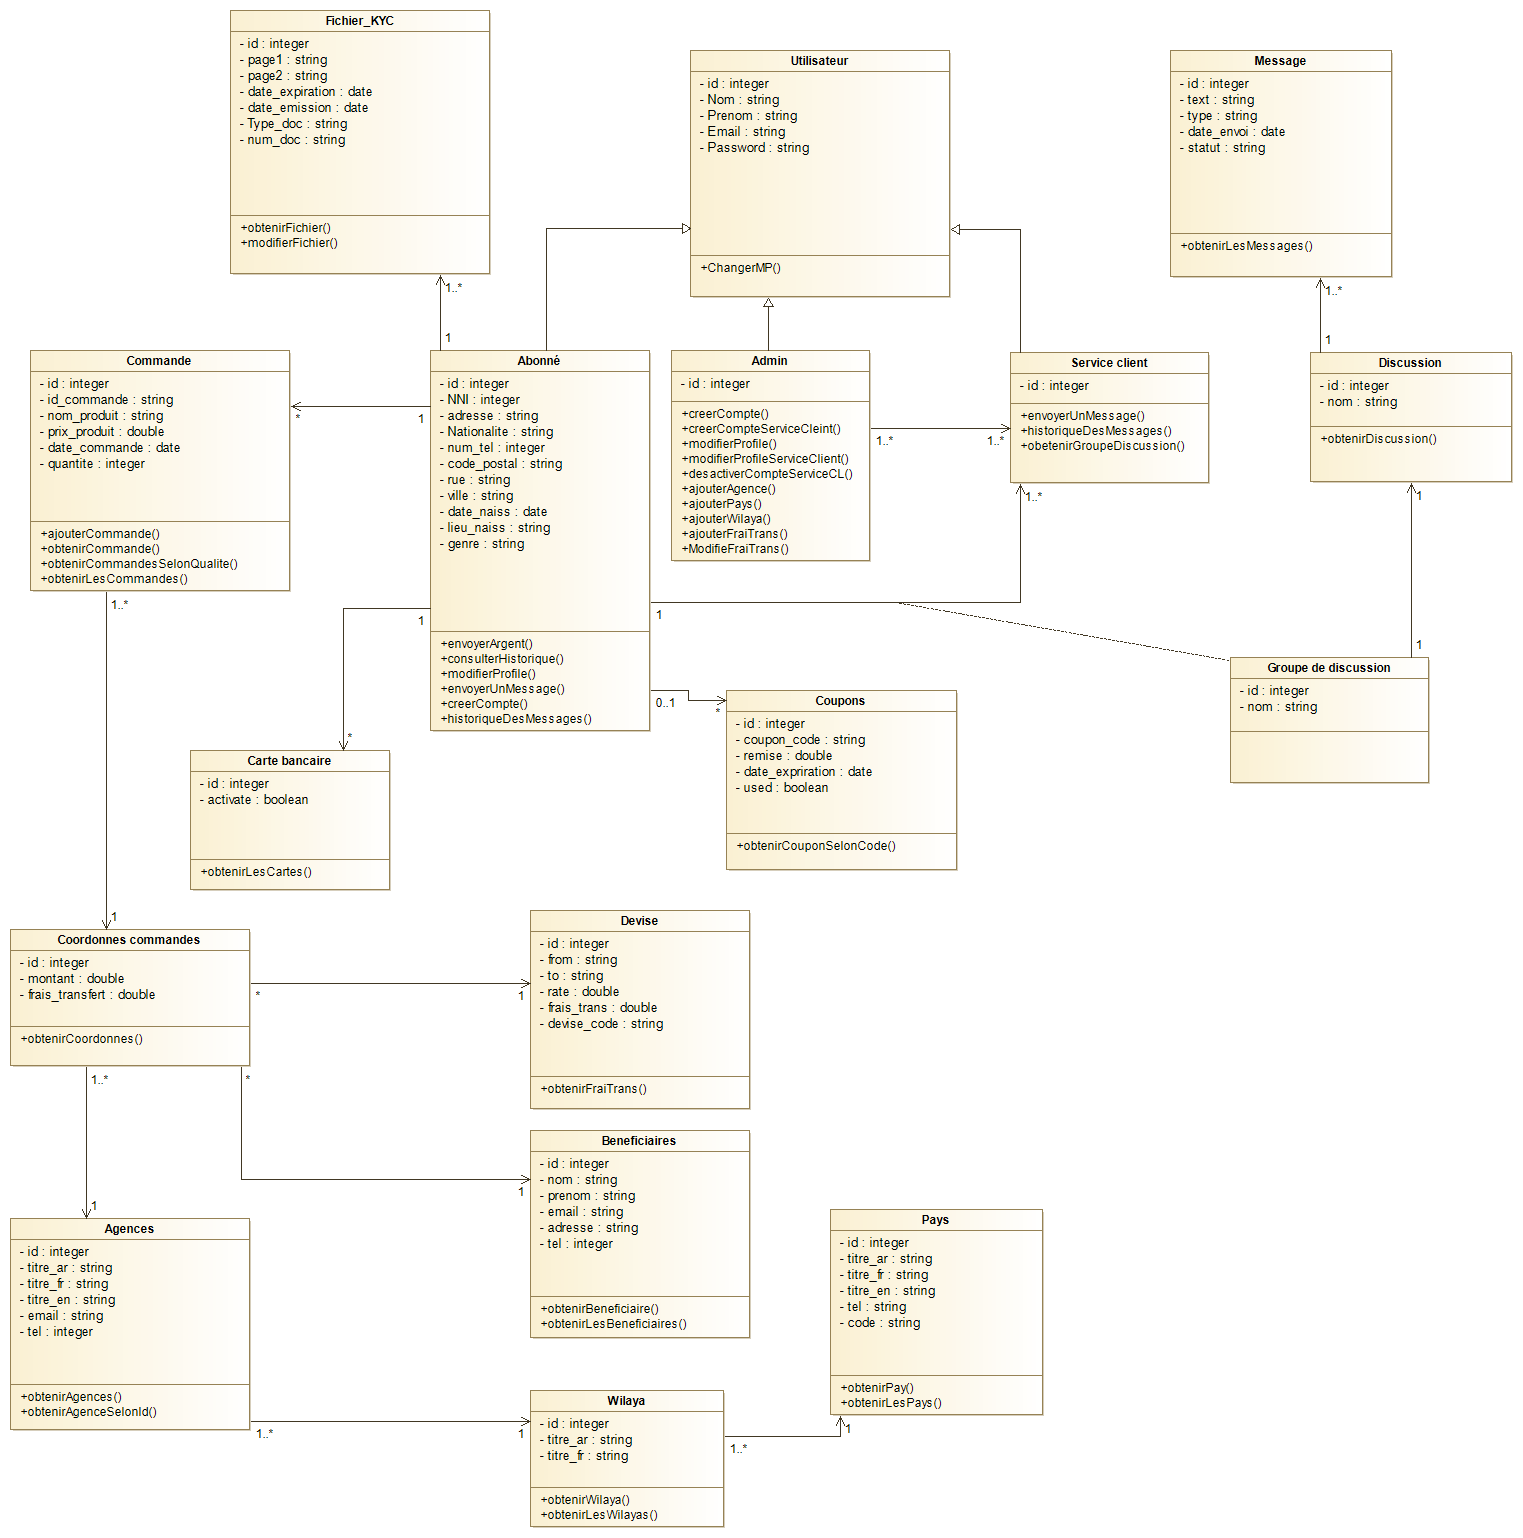
\includegraphics[width=18cm, height=20cm]{./Template LaTeX/Images/Diagramme_de_classe_V3.png}
	\caption{Diagramme de classe}
	\label{fig4:class}
\end{figure}
\newpage
\hspace*{-2cm} Le tableau~\ref{fig4:classT} explique les différentes classes de la base de données.
\begin{table}[h]
	\hspace*{-2cm}
	%\vspace*{6cm}
	\begin{tabular}{|m{5cm}|m{14cm}|}
		\hline
			\textbf{Classe}& \textbf{Description}
		\\
		\hline
		Abonné&Informations de l'utilisateur
		\\
		\hline
		Fichier KYC&  Contient les informations du fichier (carte d'identité, passeport, titre de séjour, carte bancaire) de client
		\\
			\hline
		Commande& Informations concernant une commande
		\\
			\hline
		Coordonnes commandes& Détails de chaque commande
		\\
			\hline
		Agences& Informations sur les agences de cadorim
		\\
			\hline
		Carte bancaire& Gestion de carte bancaire\\
		\hline	
			Devise& Informations sur la devise selon le pays d'envoi et le pays reçoivent
		\\
		\hline
			Beneficiaires&Informations sur les Beneficiaires
		\\
		\hline	
			Wilaya&Informations sur les Wilayas
		\\
		\hline	
			Admin&Informations de l’Admin et ses privilèges
		\\
		\hline	
			Service client&Service client avec certains privilèges
		\\
		\hline	
			Coupons&Informations d’un coupon
		\\
		\hline	
			Groupe de discussion&Informations sur les groupes
		\\
		\hline	
			Discussion&Informations de discussion de chaque groupe
		\\
		\hline		
			Message&Contient les messages de chaque discussion
		\\
		\hline
			Pays&Informations sur les pays
		\\
		\hline		
	\end{tabular}
	%\vspace*{10cm}
	\centering \caption{Description de la base de données}
	\label{fig4:classT}
\end{table}

%%%%%%%%%%%%%%%%%%%%%%%%%%%%%%%%%%%%%%%%%%%%5 ICI %%%%%%%%%%%%%%%%%%%%%%%%%%%%%%%%%%%%%%%%555

